\documentclass[11pt]{scrartcl}
\usepackage[T1]{fontenc}
\usepackage[a4paper, left=3cm, right=2cm, top=2cm, bottom=2cm]{geometry}
\usepackage[activate]{pdfcprot}
\usepackage[ngerman]{babel}
\usepackage[parfill]{parskip}
\usepackage[utf8]{inputenc}
\usepackage[math]{kurier}
\usepackage{amsmath}
\usepackage{amssymb}
\usepackage{xcolor}
\usepackage{epstopdf}
\usepackage{txfonts}
\usepackage{fancyhdr}
\usepackage{graphicx}
\usepackage{prettyref}
\usepackage{hyperref}
\usepackage{eurosym}
\usepackage{setspace}
\usepackage{units}
\usepackage{eso-pic,graphicx}
\usepackage{icomma}
\usepackage{pdfpages}

\definecolor{darkblue}{rgb}{0,0,.5}
\hypersetup{pdftex=true, colorlinks=true, breaklinks=false, linkcolor=black, menucolor=black, urlcolor=darkblue}



\setlength{\columnsep}{2cm}


\newcommand{\arcsinh}{\mathrm{arcsinh}}
\newcommand{\asinh}{\mathrm{arcsinh}}
\newcommand{\ergebnis}{\textcolor{red}{\mathrm{Ergebnis}}}
\newcommand{\fehlt}{\textcolor{red}{Hier fehlen noch Inhalte.}}
\newcommand{\betanotice}{\textcolor{red}{Diese Aufgaben sind noch nicht in der Übung kontrolliert worden. Es sind lediglich meine Überlegungen und Lösungsansätze zu den Aufgaben. Es können Fehler enthalten sein!!! Das Dokument wird fortwährend aktualisiert und erst wenn das \textcolor{black}{beta} aus dem Dateinamen verschwindet ist es endgültig.}}
\newcommand{\half}{\frac{1}{2}}
\renewcommand{\d}{\, \mathrm d}
\newcommand{\punkte}{\textcolor{white}{xxxxx}}
\newcommand{\p}{\, \partial}
\newcommand{\dd}[1]{\item[#1] \hfill \\}

\renewcommand{\familydefault}{\sfdefault}
\renewcommand\thesection{}
\renewcommand\thesubsection{}
\renewcommand\thesubsubsection{}


\newcommand{\themodul}{Messtechnik}
\newcommand{\thetutor}{Prof. Helsper}
\newcommand{\theuebung}{Übungsklausur 2}

\pagestyle{fancy}
\fancyhead[L]{\footnotesize{C. Hansen}}
\chead{\thepage}
\rhead{}
\lfoot{}
\cfoot{}
\rfoot{}

\title{\themodul{}, \theuebung{}, \thetutor}


\author{Christoph Hansen \\ {\small \href{mailto:chris@university-material.de}{chris@university-material.de}} }

\date{}


\begin{document}

\maketitle

Dieser Text ist unter dieser \href{http://creativecommons.org/licenses/by-nc-sa/4.0/}{Creative Commons} Lizenz veröffentlicht.

\textcolor{red}{Ich erhebe keinen Anspruch auf Vollständigkeit oder Richtigkeit. Falls ihr Fehler findet oder etwas fehlt, dann meldet euch bitte über den Emailkontakt.}

\tableofcontents


\newpage



\section{Aufgabe 1}

Die richtigen Antworten sind:


\begin{center}
	\begin{tabular}{c|c|c|c|c|c|c|c}
		1 & 2 & 3 & 4 & 5 & 6 & 7 & 8 \\ 
		\hline d & a & d & c & a,d & c & / & c \\  
	\end{tabular} 
\end{center}


\section{Aufgabe 2}

\subsection*{a)}

Wir haben eine Frequenz von $f = \frac{1}{\unit[5]{ms}} = \unit[200]{Hz}$

\subsection*{b)}

Die effektive Spannung können wir dann nach folgender Formel bestimmen:

\begin{align*}
	U^2 &= \frac{1}{5} \cdot \left[ 4 \cdot 20^2 + 1 \cdot \left( 40 \right)^2 \right] = \unit[3200]{\mu V^2} \\
	\hfill \\
	\Rightarrow U &= \unit[56,56]{\mu V}
\end{align*}


\subsection*{c)}

Das Gleichstrommessgerät müsste $U = \frac{4 \cdot 20 - 40}{5} = \unit[8]{\mu V}$ anzeigen.


\subsection*{d)}

Das Wechselstrommessgerät zeigt nur den Wechselanteil an:

\paragraph{Schritt 1}

Wechselspannungseinkopplung, das macht den Gleichtaktanteil zu 0.

\paragraph{Schritt 2}

Gleichrichtung

\paragraph{Schritt 3}

arithmetischer Mittelwert $\unit[24]{\mu A}$

\paragraph{Schritt 4}

Multiplikation mit Formfaktor für Sinus

\begin{align*}
U_\sim = 1,11111 \cdot 24 = \unit[26,66]{\mu V}
\end{align*}


\section{Aufgabe 3}

\subsection*{a)}


\begin{figure}[h]
	\centering
	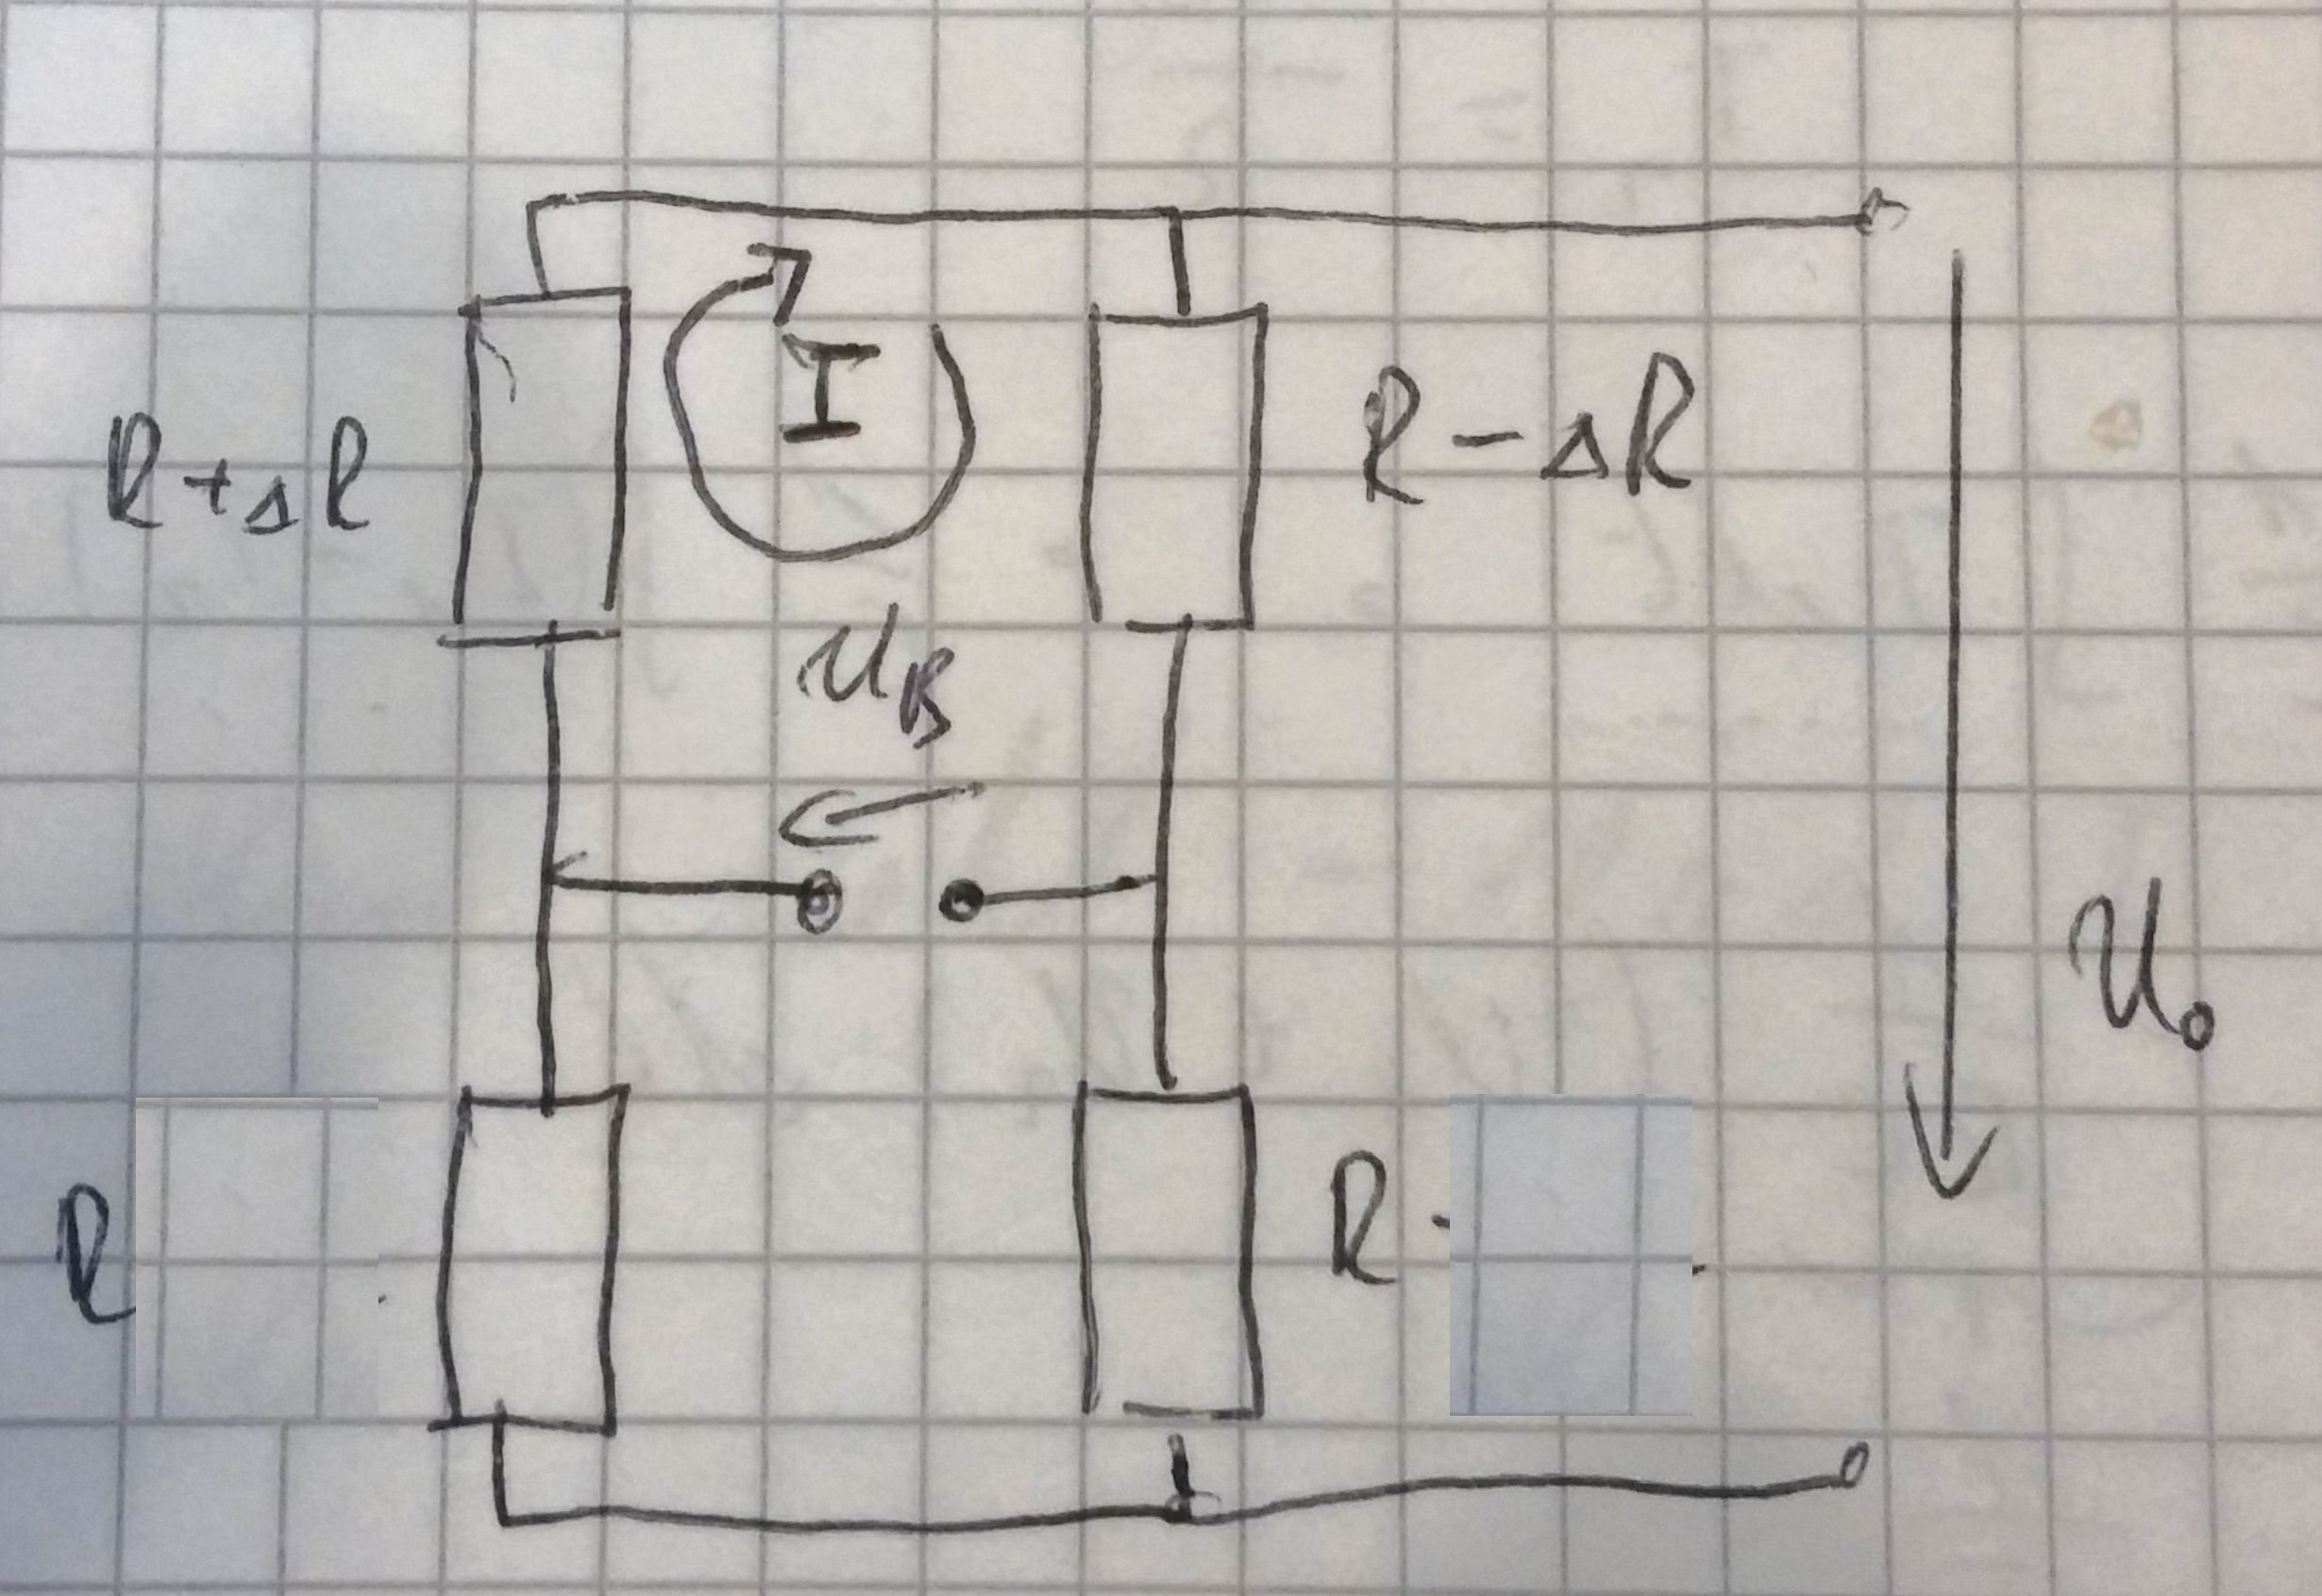
\includegraphics[scale=0.15]{A3_1.jpg}
\end{figure}


\subsection*{b)}

\begin{align*}
I_1 &= \frac{U_0}{R + \Delta R - \Delta R + R} = \frac{U_0}{2R} = I_2
\intertext{Wir betrachten nun die Masche I:}
0 &= I(R - \Delta R) + U_B - I(R + \Delta R) \\
\Leftrightarrow 0 &= \frac{U_0}{2R} \cdot R - \frac{U_0}{2R} \cdot \Delta R + U_B - \frac{U_0}{2R} \cdot R - \frac{U_0}{2R} \cdot \Delta R \\
\Leftrightarrow U_B &= \frac{\Delta R}{R} \cdot U_0
\end{align*}


\subsection*{c)}

\begin{align*}
\frac{\Delta R}{R} &= k \cdot \epsilon \\
\Leftrightarrow U_B &= k \cdot \epsilon \cdot U_O 
\intertext{Für die Empfindlichkeit müssen wir nach $\epsilon$ ableiten:}
E &= \frac{\p U_B}{\p \epsilon} = k \cdot U_0 = 2 \cdot 24 = \unit[48]{V}
\end{align*}


\section{Aufgabe 4}

\subsection*{a)}

\begin{figure}[h]
	\centering
	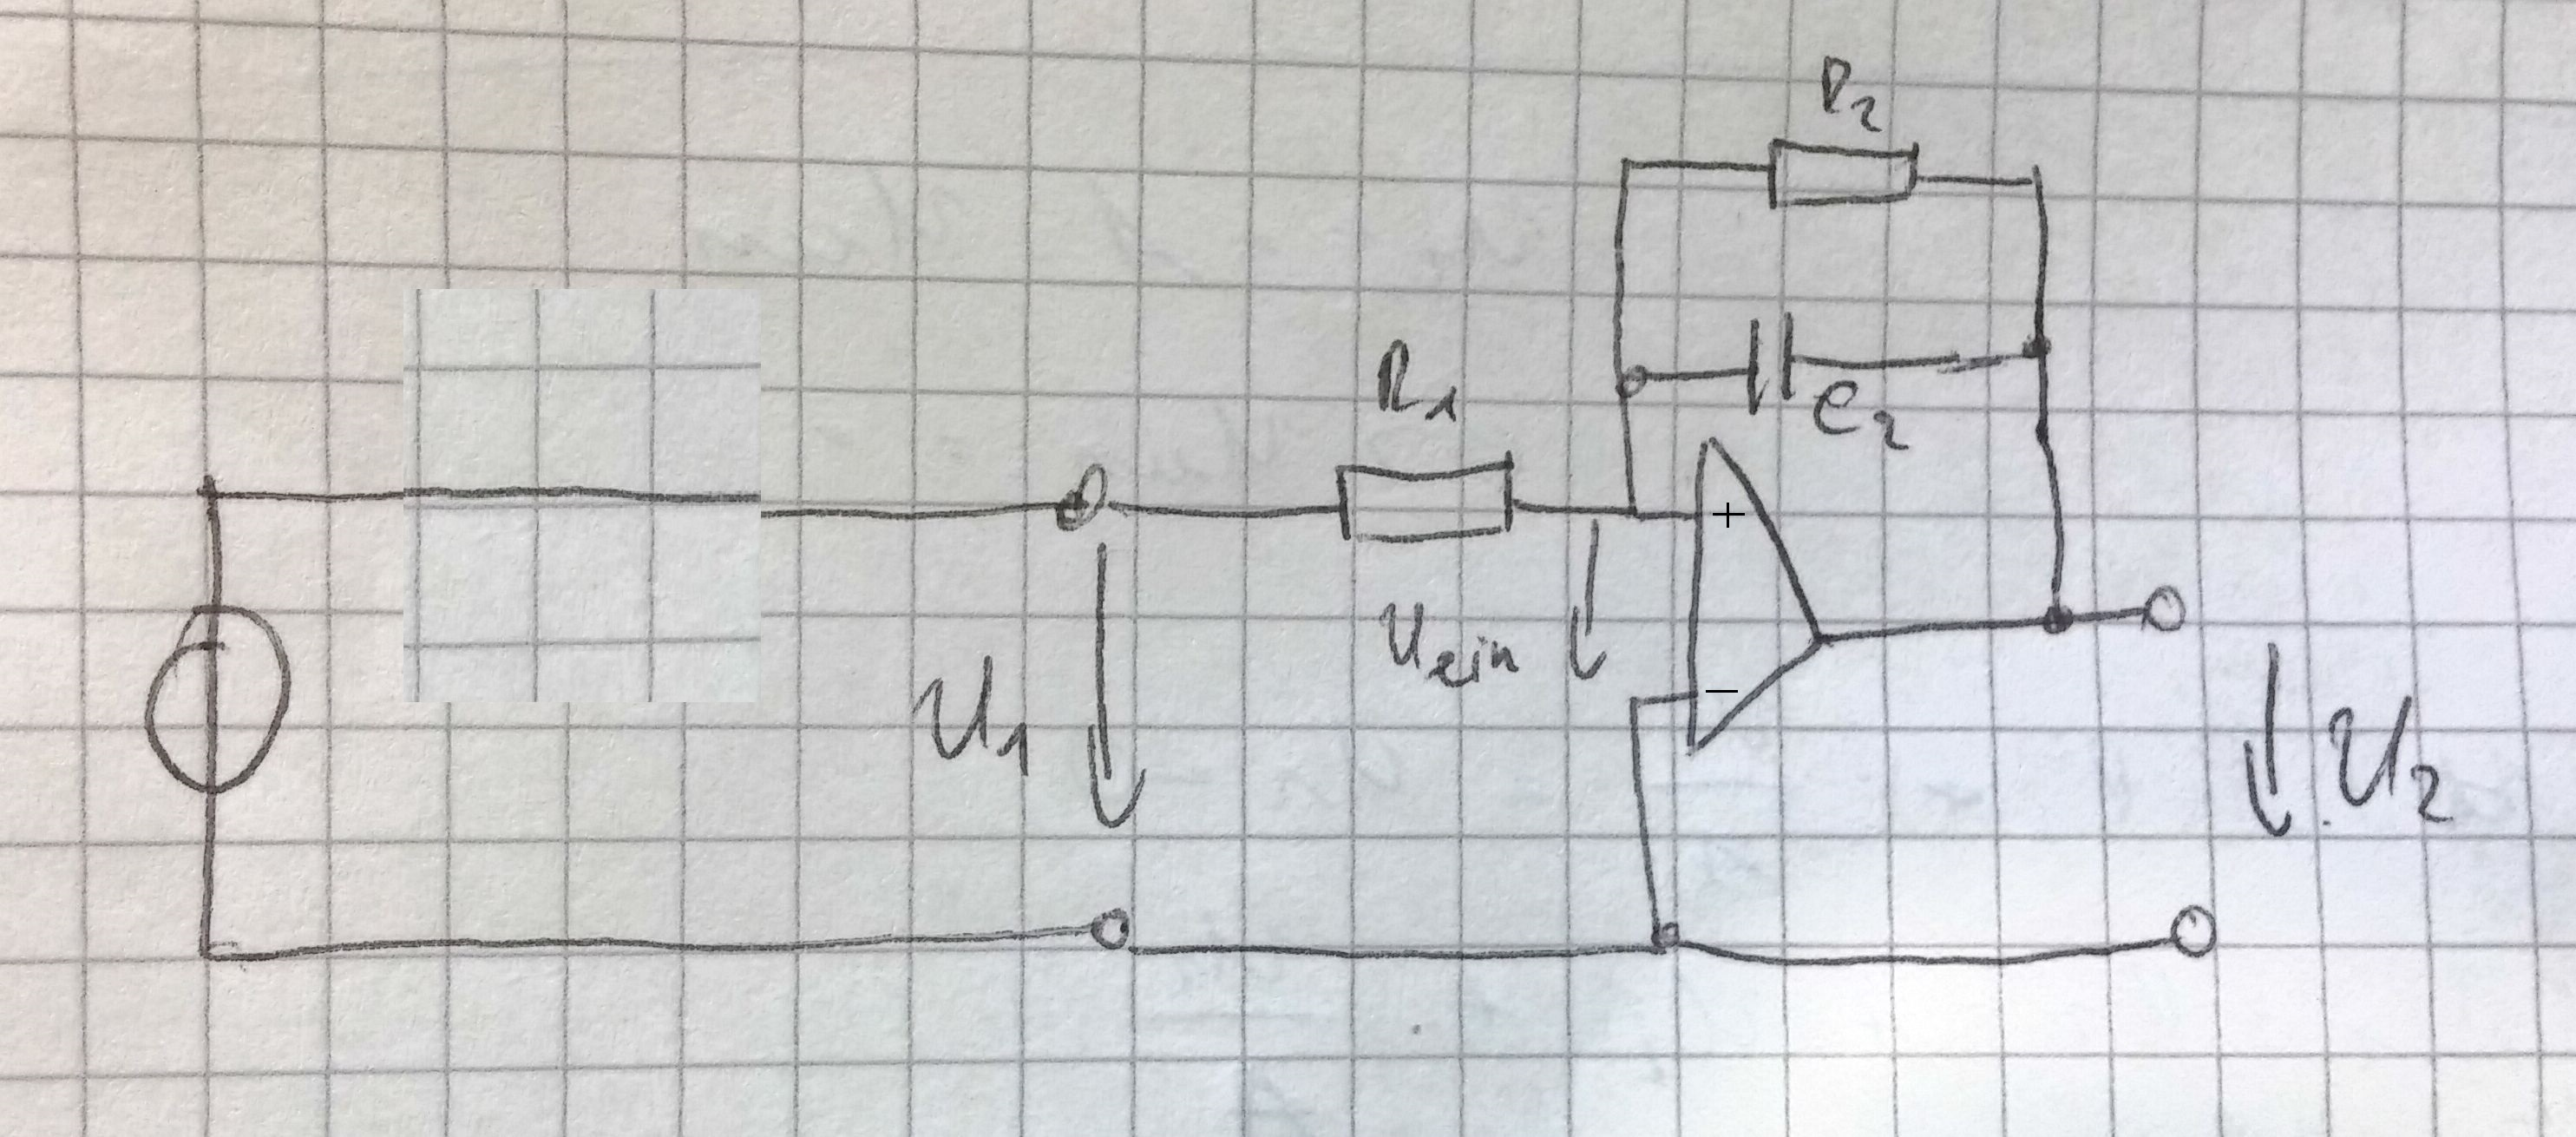
\includegraphics[scale=0.2]{A4_1.jpg}
	\caption{$U_1 = \unit[51,875]{mV}, U_2 = \unit[900]{mV}, R_1 = \unit[10]{k \Omega}$}	
\end{figure}

Mir ist allerdings nicht klar was man mit dem Biasstrom macht.

\subsection*{b)}

Zuerst bestimmen wir den Widerstand $R_2$:

\begin{align*}
\frac{R_2}{R_1} &= \frac{U_2}{U_1} \\
\Leftrightarrow R_2 &= \frac{900}{51,875} \cdot 10 = \unit[173,5]{k \Omega}
\intertext{Wir wissen, das bei der Grenzfrequenz die Verstärkung 1 ist. Darüber können wir nun die Kapazität $C_2$ ausrechnen:}
V &= \frac{R_2}{R_1} \cdot \frac{1}{1 + j \omega R_2 C_2} = 1 \\
\Leftrightarrow \frac{R_2}{R_1} - 1 &= j \omega R_2 C_2 \\
\Leftrightarrow C_2 &= \frac{\frac{R_2}{R_1} - 1}{\omega R_2} = \frac{\frac{173500}{10000} - 1}{2\pi \cdot 0,5 \cdot 173500} = \unit[30]{\mu F}
\end{align*}

\subsection*{c)}

Wir setzen in die Formel von b) ein:

\begin{align*}
V &= \frac{R_2}{R_1} \cdot \frac{1}{1 + j \omega R_2 C_2} = \frac{173500}{10000} \cdot \frac{1}{1 + 2 \pi \cdot 50 \cdot 173500 \cdot 30 \cdot 10^{-6}} \approx 1,01
\end{align*}





\end{document}